\section{GASing Implementation and Algorithms}\label{sec:methodology}

\subsection{Addition Algorithm}

The GASing addition algorithm processes numbers from left to right (most significant digit to least significant), contrary to the traditional right-to-left approach. This presents several advantages:

\begin{lstlisting}[language=Python, caption=GASing Addition Algorithm]
function GASing_Addition(a, b):
    result = ""
    carry = 0
    
    # Pad the shorter number with leading zeros
    a = pad_with_zeros(a, len(b))
    b = pad_with_zeros(b, len(a))
    
    # Process from left to right
    for i in range(0, len(a)):
        # Add digits and carry
        digit_sum = int(a[i]) + int(b[i]) + carry
        
        # Determine new digit and carry
        if digit_sum > 9:
            carry = 1
            digit = digit_sum - 10
        else:
            carry = 0
            digit = digit_sum
            
        result += str(digit)
    
    # Add final carry if necessary
    if carry > 0:
        result += str(carry)
        
    return result
\end{lstlisting}

The left-to-right processing allows for:
\begin{itemize}
    \item Earlier termination for approximate calculations
    \item Alignment with human reading order
    \item Potential parallelization in computational contexts
\end{itemize}

\subsection{Multiplication Algorithm}

GASing multiplication extends the addition algorithm through a structured grid approach:

\begin{lstlisting}[language=Python, caption=GASing Multiplication Algorithm]
function GASing_Multiplication(a, b):
    # Initialize result grid
    rows = len(b)
    cols = len(a)
    grid = initialize_grid(rows, cols)
    
    # Fill multiplication grid
    for i in range(rows):
        for j in range(cols):
            grid[i][j] = int(b[i]) * int(a[j])
    
    # Apply carry propagation using pattern recognition
    apply_carries(grid)
    
    # Convert grid to result
    result = grid_to_result(grid)
    
    return result
\end{lstlisting}

The grid-based approach facilitates:
\begin{itemize}
    \item Visualization of the multiplication process
    \item Systematic carry handling
    \item Identification of patterns in partial products
\end{itemize}

\subsection{Subtraction and Division}

Subtraction in GASing employs the complement method, where negative results at any position trigger borrowing operations in a systematic way. Division extends subtraction through iterative processes with optimization for common patterns.

<<<<<<< HEAD
\subsection{Problem Definition}

[Define the specific problem you are addressing with your Petri Net model]

\subsection{Proposed Petri Net Model}

Our proposed Petri Net model for [specific system or process] consists of the following components:

\begin{itemize}
    \item \textbf{Places}: Represent [specific states or conditions in your system]
    \item \textbf{Transitions}: Represent [specific events or actions in your system]
    \item \textbf{Tokens}: Represent [specific resources or entities in your system]
\end{itemize}

\begin{figure}[htbp]
\centering
\begin{tikzpicture}[node distance=1.5cm and 2.5cm, >=stealth, bend angle=45, auto] % Adjusted default node distances

% Define places with new coordinates for better layout
\placewithtokens{p1}{0,0}{2}        % Resource
\placewithtokens{p2}{5,0}{0}        % Process
\placewithtokens{p3}{2.5,-2.5}{1}    % Control
\placewithtokens{p4}{7.5,-2.5}{0}    % Output
\placewithtokens{p5}{2.5,-5.5}{0}    % Complete

% Define transitions with new coordinates
\node[transition] (t1) at (2.5,0) {};   % Start (between P1 and P2, above P3)
\node[transition] (t2) at (5,-2.5) {};  % Execute (between P2 and P4, aligned with P3)
\node[transition] (t3) at (1,-4) {};    % Cancel (below and to the left of P3, leading to P5)
\node[transition] (t4) at (4,-4) {};    % Finish (below and to the right of P3, or below T2, leading to P5)

% Define arcs (connections remain logically the same)
\draw[pre] (p1) -- (t1);
\draw[post] (t1) -- (p2);
\draw[pre] (p3) -- (t1);    % P3 is an input to T1
\draw[post] (t1) -- (p3);   % T1 returns a token to P3 (maintains control token)

\draw[pre] (p2) -- (t2);
\draw[pre] (p3) -- (t2);    % P3 is also an input to T2
\draw[post] (t2) -- (p4);

\draw[pre] (p3) -- (t3);
\draw[post] (t3) -- (p5);

\draw[pre] (p4) -- (t4);
\draw[post] (t4) -- (p5);

% Add labels (node anchors ensure they are placed relative to the node)
\node[above] at (p1.north) {Resource};
\node[above] at (p2.north) {Process};
\node[left] at (p3.west) {Control}; % Adjusted to left to avoid overlap with T1-P3 arc
\node[above] at (p4.north) {Output}; % Adjusted to above for consistency
\node[below] at (p5.south) {Complete};

\node[above] at (t1.north) {Start};
\node[above] at (t2.north) {Execute}; % Adjusted to above
\node[left] at (t3.west) {Cancel};
\node[right] at (t4.east) {Finish};

% Add a title
\node[above=1cm of p1.north -| t1.north] {Petri Net Model of a Simple Workflow Process}; % Position title relative to top elements

\end{tikzpicture}
\caption{Generic Petri Net model structure for [specific system or process]}
\label{fig:petri_net_generic_model}
\end{figure}

To illustrate common concurrency problems that can be modeled with Petri Nets, we present the Dining Philosophers problem (Figure \ref{fig:dining_philosophers}) and the Producer-Consumer problem (Figure \ref{fig:producer_consumer_workflow}).

\begin{figure*}[htbp]
\centering
% Petri Net Model of the Dining Philosophers Problem (Refined)
\begin{tikzpicture}[node distance=2.2cm and 2.2cm, >=stealth, bend angle=30, auto, on grid]
    % Philosopher thinking states
    \placewithtokens{p1}{0,0}{1}
    \placewithtokens{p2}{3,0}{1}
    \placewithtokens{p3}{1.5,-2.6}{1}

    % Philosopher eating states
    \placewithtokens{e1}{-1.2,-1.5}{0}
    \placewithtokens{e2}{4.2,-1.5}{0}
    \placewithtokens{e3}{1.5,-4.1}{0}

    % Forks
    \placewithtokens{f1}{0,-1.5}{1}
    \placewithtokens{f2}{3,-1.5}{1}
    \placewithtokens{f3}{1.5,-1.5}{1}

    % Transitions (pick up forks)
    \node[transition, rounded corners=2pt] (t1) [below left=0.7cm and 0.7cm of p1] {};
    \node[transition, rounded corners=2pt] (t2) [below right=0.7cm and 0.7cm of p2] {};
    \node[transition, rounded corners=2pt] (t3) [below=0.7cm of p3] {};

    % Transitions (put down forks)
    \node[transition, rounded corners=2pt] (r1) [left=1.2cm of e1] {};
    \node[transition, rounded corners=2pt] (r2) [right=1.2cm of e2] {};
    \node[transition, rounded corners=2pt] (r3) [below=1.2cm of e3] {};

    % Arcs for Philosopher 1
    \draw[pre] (p1) -- (t1);
    \draw[pre] (f1) -- (t1);
    \draw[pre] (f3) -- (t1);
    \draw[post] (t1) -- (e1);
    \draw[pre] (e1) -- (r1);
    \draw[post] (r1) -- (p1);
    \draw[post] (r1) -- (f1);
    \draw[post] (r1) -- (f3);

    % Arcs for Philosopher 2
    \draw[pre] (p2) -- (t2);
    \draw[pre] (f2) -- (t2);
    \draw[pre] (f3) -- (t2);
    \draw[post] (t2) -- (e2);
    \draw[pre] (e2) -- (r2);
    \draw[post] (r2) -- (p2);
    \draw[post] (r2) -- (f2);
    \draw[post] (r2) -- (f3);

    % Arcs for Philosopher 3
    \draw[pre] (p3) -- (t3);
    \draw[pre] (f1) -- (t3);
    \draw[pre] (f2) -- (t3);
    \draw[post] (t3) -- (e3);
    \draw[pre] (e3) -- (r3);
    \draw[post] (r3) -- (p3);
    \draw[post] (r3) -- (f1);
    \draw[post] (r3) -- (f2);

    % Labels for philosophers
    \node[above] at (p1.north) {P1 thinking};
    \node[above] at (p2.north) {P2 thinking};
    \node[below] at (p3.south) {P3 thinking};
    \node[left] at (e1.west) {P1 eating};
    \node[right] at (e2.east) {P2 eating};
    \node[below] at (e3.south) {P3 eating};

    % Labels for forks
    \node[below left] at (f1.south west) {Fork 1};
    \node[below right] at (f2.south east) {Fork 2};
    \node[above] at (f3.north) {Fork 3};

    % Title
    \node[above=1cm] at (current bounding box.north) {Petri Net Model of the Dining Philosophers Problem};
\end{tikzpicture}
\caption{Petri Net model of the Dining Philosophers problem}
\label{fig:dining_philosophers}
\end{figure*}

% First instance of linear_petri_net as a resized figure
\begin{figure}[htbp]
\centering
\resizebox{0.88\columnwidth}{!}{\begin{tikzpicture}[every place/.style={minimum size=10mm}, node distance=1.7cm]
  % Places
  \node[place] (A) {$A$};
  \node[transition] (fa) [right of=A] {$f_1^X$};
  \node[place] (B) [right of=fa] {$B$};
  \node[transition] (fb) [right of=B] {$f_b$};
  \node[place] (C) [right of=fb] {$C$};
  \node[transition] (fc) [right of=C] {$f_c$};
  \node[place] (Y) [right of=fc] {$Y$};

  % Arcs
  \draw[->] (A) -- (fa);
  \draw[->] (fa) -- (B);
  \draw[->] (B) -- (fb);
  \draw[->] (fb) -- (C);
  \draw[->] (C) -- (fc);
  \draw[->] (fc) -- (Y);
\end{tikzpicture}}
\caption{Resized Linear Petri Net}
\label{fig:linear_petri_resized}
\end{figure}

% Second instance as a regular figure
\begin{figure}[htbp]
\centering
\begin{tikzpicture}[every place/.style={minimum size=10mm}, node distance=1.7cm]
  % Places
  \node[place] (A) {$A$};
  \node[transition] (fa) [right of=A] {$f_1^X$};
  \node[place] (B) [right of=fa] {$B$};
  \node[transition] (fb) [right of=B] {$f_b$};
  \node[place] (C) [right of=fb] {$C$};
  \node[transition] (fc) [right of=C] {$f_c$};
  \node[place] (Y) [right of=fc] {$Y$};

  % Arcs
  \draw[->] (A) -- (fa);
  \draw[->] (fa) -- (B);
  \draw[->] (B) -- (fb);
  \draw[->] (fb) -- (C);
  \draw[->] (C) -- (fc);
  \draw[->] (fc) -- (Y);
\end{tikzpicture}
\caption{Tensorized Petri Net Structure}
\label{fig:tensor_petri}
\end{figure}

\begin{figure}[htbp]
% Petri Net Model of the Producer-Consumer Problem (Refined)
\begin{tikzpicture}[node distance=2.2cm and 2.2cm, >=stealth, bend angle=30, auto, on grid]
    % Places
    \placewithtokens{producer}{0,0}{1}
    \placewithtokens{buffer}{2.8,0}{0}
    \placewithtokens{consumer}{5.6,0}{1}
    \placewithtokens{bufferCapacity}{2.8,-2.2}{3}

    % Transitions
    \node[transition, rounded corners=2pt] (produce) [right=of producer] {};
    \node[transition, rounded corners=2pt] (consume) [right=of buffer] {};

    % Arcs
    \draw[pre] (producer) -- (produce);
    \draw[post] (produce) -- (producer);
    \draw[post] (produce) -- (buffer);
    \draw[pre] (buffer) -- (consume);
    \draw[pre] (consumer) -- (consume);
    \draw[post] (consume) -- (consumer);
    \draw[pre] (bufferCapacity) -- (produce);
    \draw[post] (consume) -- (bufferCapacity);

    % Labels
    \node[above] at (producer.north) {Producer};
    \node[above] at (buffer.north) {Buffer};
    \node[above] at (consumer.north) {Consumer};
    \node[below] at (bufferCapacity.south) {Buffer Capacity};
    \node[above] at (produce.north) {Produce};
    \node[above] at (consume.north) {Consume};

    % Title
    \node[above=1cm] at (current bounding box.north) {Petri Net Model of the Producer-Consumer Problem};
\end{tikzpicture}
\caption{Producer-Consumer Workflow}
\label{fig:producer_consumer_workflow}
\end{figure}

\begin{figure}[htbp]
\centering
\begin{tikzpicture}[every place/.style={minimum size=10mm}, node distance=1.7cm and 2.2cm]
  % First digit addition
  \node[place] (a1) {$a_1$};
  \node[place, below of=a1] (b1) {$b_1$};
  \node[place, below of=b1] (c0) {$c_0$};
  \node[transition] (add1) [right of=b1, yshift=1.1cm] {$+_1$};
  \node[place] (s1) [right of=add1, yshift=0.8cm] {$s_1$};
  \node[place] (c1) [below of=s1] {$c_1$};

  \draw[->] (a1) -- (add1);
  \draw[->] (b1) -- (add1);
  \draw[->] (c0) -- (add1);
  \draw[->] (add1) -- (s1);
  \draw[->] (add1) -- (c1);

  % Second digit addition
  \node[place, below of=c1] (a2) {$a_2$};
  \node[place, below of=a2] (b2) {$b_2$};
  \node[transition] (add2) [right of=b2, yshift=1.1cm] {$+_2$};
  \node[place] (s2) [right of=add2, yshift=0.8cm] {$s_2$};
  \node[place] (c2) [below of=s2] {$c_2$};

  \draw[->] (a2) -- (add2);
  \draw[->] (b2) -- (add2);
  \draw[->] (c1) -- (add2);
  \draw[->] (add2) -- (s2);
  \draw[->] (add2) -- (c2);
\end{tikzpicture}
\caption{Carry Arithmetic as Feedback System.}
\label{fig:carry_arithmetic_feedback}
\end{figure}

\begin{figure}[htbp]
\centering
\resizebox{0.9\columnwidth}{!}{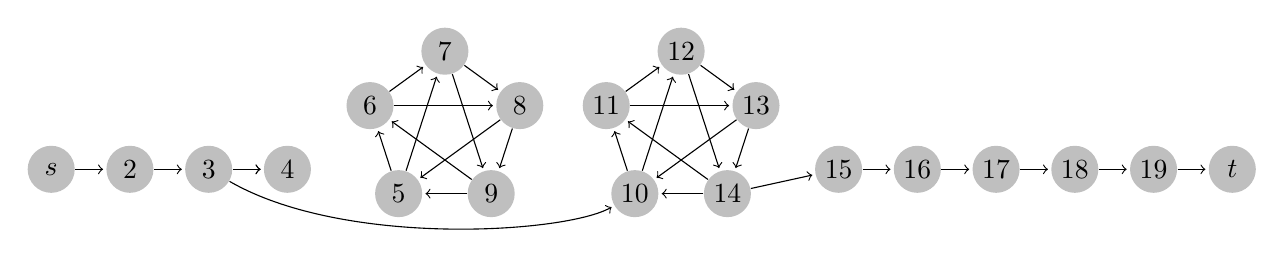
\begin{tikzpicture}
    [shorten >=1pt,->,
     vertex/.style={circle,fill=black!25,minimum size=17pt,inner sep=0pt}]
  
    \foreach \name/\x in {s/1, 2/2, 3/3, 4/4, 15/11, 16/12, 17/13, 18/14, 19/15, t/16}
      \node[vertex] (G-\name) at (\x,0) {$\name$};
  
    \foreach \name/\angle/\text in {P-1/234/5, P-2/162/6, P-3/90/7, P-4/18/8, P-5/-54/9}
      \node[vertex,xshift=6cm,yshift=.5cm] (\name) at (\angle:1cm) {$\text$};
  
    \foreach \name/\angle/\text in {Q-1/234/10, Q-2/162/11, Q-3/90/12, Q-4/18/13, Q-5/-54/14}
      \node[vertex,xshift=9cm,yshift=.5cm] (\name) at (\angle:1cm) {$\text$};
  
    \foreach \from/\to in {s/2,2/3,3/4,3/4,15/16,16/17,17/18,18/19,19/t}
      \draw (G-\from) -- (G-\to);
  
    \foreach \from/\to in {1/2,2/3,3/4,4/5,5/1,1/3,2/4,3/5,4/1,5/2}
      { \draw (P-\from) -- (P-\to); \draw (Q-\from) -- (Q-\to); }
  
    \draw (G-3) .. controls +(-30:2cm) and +(-150:1cm) .. (Q-1);
    \draw (Q-5) -- (G-15);
  \end{tikzpicture}}
\caption{Example of a complex graph structure with cycles and cross-connections.}
\label{fig:complex_graph_example}
\end{figure}

\subsection{Model Analysis}

To analyze the properties of our Petri Net model, we examine:
=======
\begin{figure}[H]
    \centering
    \begin{tikzpicture}
        % Addition operation diagram showing digit-wise processing
        \node[operation, minimum width=4cm] (addition) at (0,0) {GASing Addition};
        \node[operation] (subtraction) at (-2.5,-2) {GASing Subtraction};
        \node[operation] (multiplication) at (2.5,-2) {GASing Multiplication};
        \node[operation, minimum width=4cm] (division) at (0,-4) {GASing Division};
        
        % Connections
        \draw[->, thick] (addition) -- (subtraction);
        \draw[->, thick] (addition) -- (multiplication);
        \draw[->, thick] (subtraction) -- (division);
        \draw[->, thick] (multiplication) -- (division);
    \end{tikzpicture}
    \caption{Hierarchical relationship between GASing arithmetic operations}
    \label{fig:gasing_operations}
\end{figure}

Our implementation architecture includes variants in multiple programming languages to facilitate performance comparisons:
>>>>>>> 81a8f8d (Added the argument for resource sensitive interpretability)

\begin{itemize}
    \item Pure Python implementations (gasing\_simulasi, penjumlahan\_tradisional)
    \item Optimized C bindings (gasing\_add\_c, gasing\_add\_c\_optimized)
    \item Rust implementations (gasing\_add\_rust, gasing\_add\_rust\_optimized)
    \item Pattern-specific optimizations for common number patterns
\end{itemize}
<<<<<<< HEAD

\subsection{Wiring Diagram Representation}

Figure \ref{fig:clock_with_display} presents a wiring diagram in the style of David Jaz Myers' work on Dynamical Systems, illustrating the structure of a clock system with display components.

\begin{figure}[htbp]
\centering
% ClockWithDisplay in Spivak/Fong style using oriented WD
\begin{tikzpicture}[oriented WD, bbx=1.2cm, bby=2ex, bb min width=2cm, bb port length=4pt, bb port sep=1.5]
    % Clock and Meridiem boxes with proper ports and more rounded corners
    % The notation bb={in}{out} specifies number of input and output ports
    \node[bb={0}{1}, fill=blue!15, thick, rounded corners=6pt] (clock) at (0, -2) {\footnotesize Clock};
    \node[bb={1}{1}, fill=blue!15, thick, rounded corners=6pt] (meridiem) at (0, 2) {\footnotesize Meridiem};
    
    % Container box that encompasses both components with more spacing
    \node[bb={0}{2}, fit={($(clock.south west)+(-0.8,-0.5)$) ($(meridiem.north east)+(0.8,0.5)$)}, thick] (container) {};
    
    % Connection from right of Clock to left of Meridiem
    % Symmetric S-curve for Clock→Meridiem (canonical categorical style)
    \draw
      (clock.east)
      .. controls ($(clock.east)+(2,2.8)$) and ($(meridiem.west)+(-2,-2.8)$)
      .. (meridiem.west);

    
    % Connect ports to container edges for outputs
    \draw (meridiem_out1) to (container_out1');
    \draw (clock_out1) to (container_out2');
    
    % External labels with better positioning
    \node[anchor=west, font=\footnotesize] at ($(container_out1)+(0.2,0)$) {a.m./p.m.};
    \node[anchor=west, font=\footnotesize] at ($(container_out2)+(0.2,0)$) {Hour};
    
    % Title below container with better spacing
    \node[font=\normalsize] at ($(container.south)+(0,0.5)$) {ClockWithDisplay};
\end{tikzpicture}
\caption{Wiring diagram of a clock with display components, showing the meridiem and hour display units.}
\label{fig:clock_with_display}
\end{figure}

\subsection{Implementation}

[Describe the tools or methods used to implement and analyze your Petri Net model]
=======
>>>>>>> 81a8f8d (Added the argument for resource sensitive interpretability)
